\chapter{测试与实验}

\section{测试总述}
本章节包含了对本文所带的样例实现进行简单测试的过程和结果。测试主要通过对客户端库进行数个集成的测试,而服务端不包含单独的测试。对服务端的测试被包含在对客户端库的测试中,通过对网络通信函数的测试来间接完成。对每个测试本章节亦会给出其对应的基准测试结果。

\section{测试环境描述}

\subsection{系统环境}

\begin{itemize}
    \item 操作系统:Arch Linux(Rolling)\footnote{即滚动性发行,所有软件包总是上游最新的};
    \item Golang 工具链:版本 1.20.4,Arch 软件包仓库版本 \verb|go 2:1.20.4-1|;
    \item 处理器:AMD Ryzen 9 4900HS with Radeon Graphics (16) @ 3.000GHz;
    \item 内存:16 GB,以及 32 GB 的 Linux 交换空间;
\end{itemize}

\subsection{样例实现使用的第三方库}

以下为本方案所使用的第三方库列表。其中,\verb|github.com/tuneinsight/lattigo/v4| 为本方案的核心库,其余为辅助库。

\begin{minted}{go}
require (
    github.com/tuneinsight/lattigo/v4 v4.1.0
    github.com/urfave/cli/v2 v2.25.1

    github.com/google/uuid v1.3.0
    github.com/kr/pretty v0.3.1
    github.com/mattn/go-sqlite3 v1.14.16
    github.com/pkg/errors v0.9.1
)
\end{minted}

\section{测试样例描述}

本方案编写了如下测试函数,其中每个测试函数都有对应的性能基准测试函数\footnote{测试操作对象 \texttt{*testing.T} 被简化为 \texttt{*T},对 \texttt{*testing.B} 同理}:

\begin{itemize}
    \item \verb|func TestCKKSEncryptAndDecrypt(*T)|:对本文代码封装的 CKKS 加密和解密函数进行正确性测试;
    \item \verb|func TestTransferBySenderPK(*T)|:测试能否正确生成交易;
    \item \verb|func TestTransferByReceiptPK(*T)|:同上;
    \item \verb|func TestAcceptTransactionByTransaction(*T)|:测试能否正确生成确认消息;
    \item \verb|func TestRegisterUser(*T)|:测试生成密钥对,将用户信息提交给服务端的功能,并且测试服务端是否能够正确地将用户信息存储到数据库中而不报出异常;
    \item \verb|func TestRegisterSwk(*T)|:在上述函数基础上,测试生成交换密钥,并将其提交给服务端;
    \item \verb|func TestCreateTransferJobBySenderPK(*T)|:在上述函数基础上,测试能否正确向服务端提交交易信息,以及服务端是否会正确响应请求;
    \item \verb|func TestCreateTransferJobByReceiptPK(*T)|:同上,但是测试的是以收款方公钥加密的密文发起的交易,涉及了双方签名和确认的过程,总共两次网络交互;
    \item \verb|func BenchmarkReEncryptCTWithSwk(*B)|:对重加密性能进行评估的基准测试函数;
    \item \verb|func TestGetUpdatedSenderBalance(*T)|:对密态余额操作进行测试和性能评估的函数;
    \item \verb|func TestGetUpdatedReceiptBalance(*T)|:同上;
\end{itemize}

以及以下的辅助函数:

\begin{itemize}
    \item \verb|func initTestRandomUser()|:准备单次测试环境,包括全局变量等。
    \item \verb|func makeNewRandomUser(string)|:生成随机用户。
\end{itemize}

\section{实验和基准测试结果}

\subsection{简单测试}

本文在测试时,使用下述命令,调用 Golang 工具链提供测试功能,对方案进行功能测试和性能测试。

\begin{minted}{shell}
$ go run ./cmd/server # 使服务端上线

# 进行集成测试
$ /usr/bin/go test -v \
  ./internal/{clientlib,serverlib}

# 进行基准性能测试
$ /usr/bin/go test \
  -bench . ./internal/{clientlib,serverlib}
\end{minted}

以 VSCode 的 Golang 插件,执行的测试输出如下图\ref{Fig:test} \ref{Fig:benchmark}所示。 

\begin{figure}
    \centering
    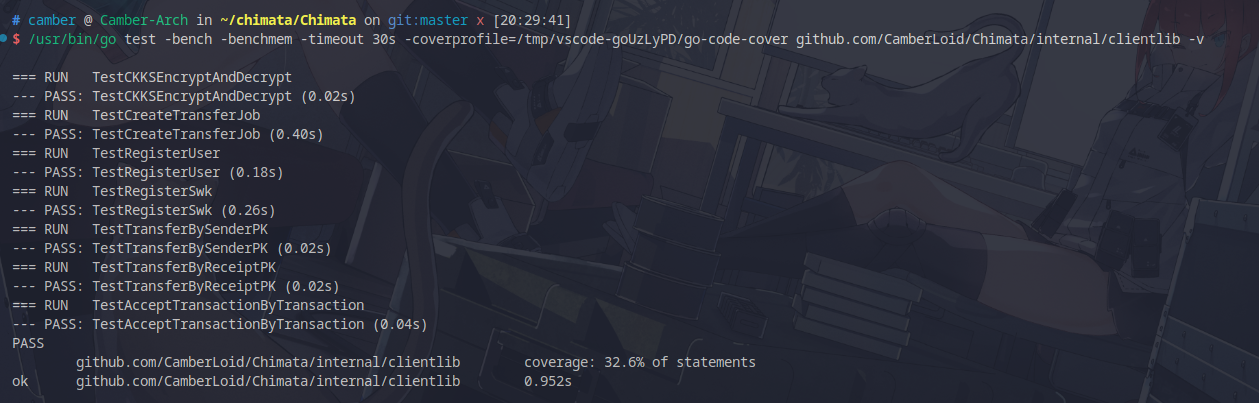
\includegraphics[width=0.7\linewidth]{./Figures/Test.png}
    \caption{以默认参数执行的集成测试输出}\label{Fig:test}
\end{figure}

\begin{figure}
    \centering
    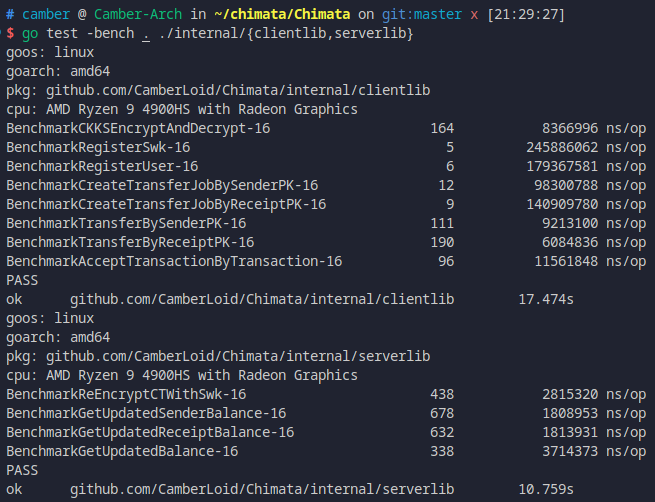
\includegraphics[width=0.7\linewidth]{./Figures/Bench_Overall.png}
    \caption{以默认参数执行的性能测试输出}\label{Fig:benchmark}
\end{figure}

\subsection{交易的时间开销测试}

\subsubsection{测试记录}

本节对完整执行一次交易的过程进行了性能的测试,包括对以发送者公钥加密密文进行的交易提出测试函数 \verb|TestTransferBySenderPK| 和以接收者公钥加密密文,并需要接收者标记接受的交易提出和确认函数 \verb|TestTransferByReceiptPK| 等,其测试结果输出如图 \ref{Fig:bench_transaction} 所示。

\begin{figure}
    \centering
    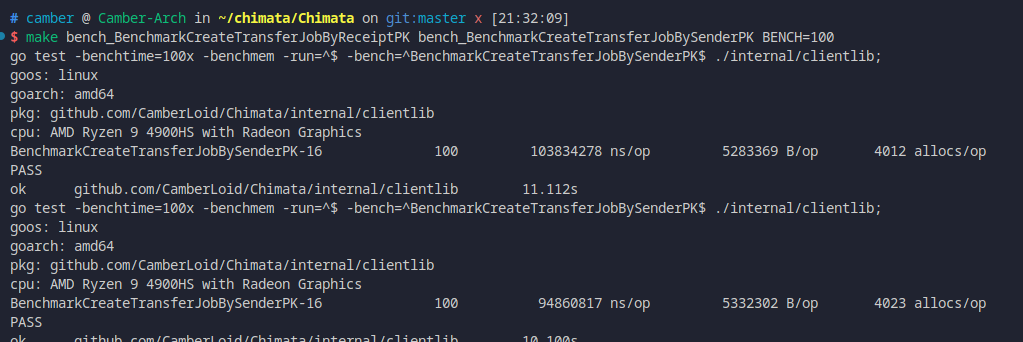
\includegraphics[width=0.8\linewidth]{./Figures/Bench_Transaction_all.png}
    \caption{交易基准测试输出}\label{Fig:bench_transaction}
\end{figure}

此外,由于 \verb|TestTransferByReceiptPK| 所涵盖的方面较为全面,包括多次 CKKS 方案的加解密和签名验证,以及对数据库的查询、插入和修改等,具有代表性,因此笔者亦对该函数的的连续执行不同次数的时间开销的实验结果进行收集,使用 Python 模组 matplotlib 绘制折线图如图\ref{Fig:graph_bench_transaction}所示。

\begin{figure}
    \centering
    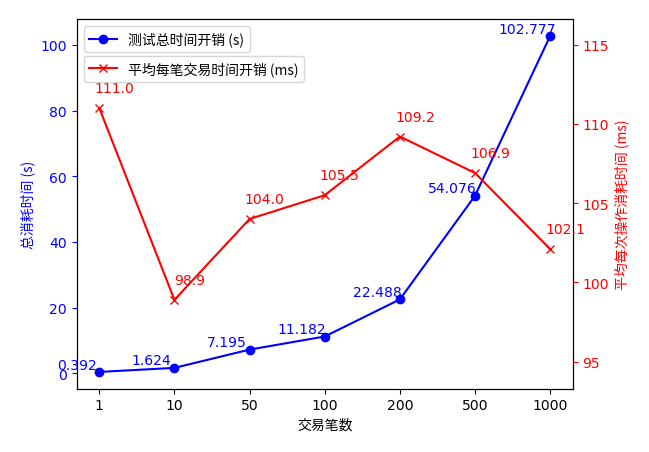
\includegraphics[width=0.8\linewidth]{./Figures/matplots/Bench_CreateTransferJobByReceiptPK.png}
    \caption{TestTransferByReceiptPK 的测试数据}\label{Fig:graph_bench_transaction}
\end{figure}

测试过程中的服务端输出如图\ref{Fig:server}所示。

\begin{figure}
    \centering
    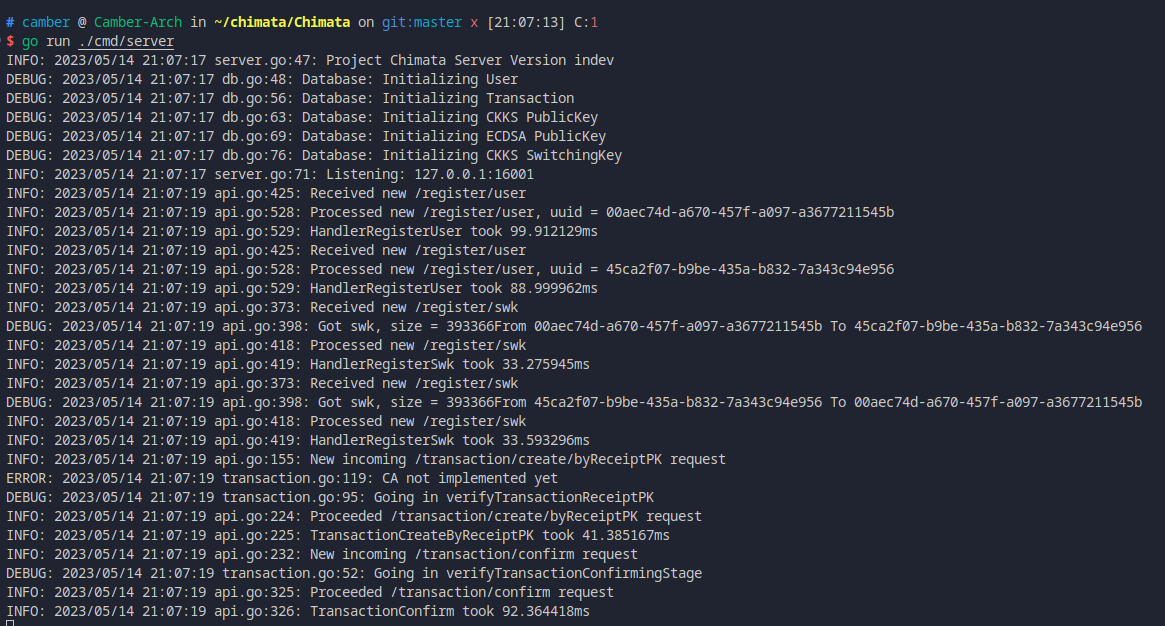
\includegraphics[width=0.8\linewidth]{./Figures/Server_ReceiptPK.png}
    \caption{服务端日志输出}\label{Fig:server}
\end{figure}

在涉及网络交互的部分之外,本文也对加解密性能和重加密性能进行了简单的评估测试。测试结果如图\ref{Fig:benchmark}和图\ref{Fig:bench_reencrypt}所示,平均每次加解密时间总和约为 12 ms,而重加密的时间开销约为 3 ms。

\begin{figure}[h]
    \centering
    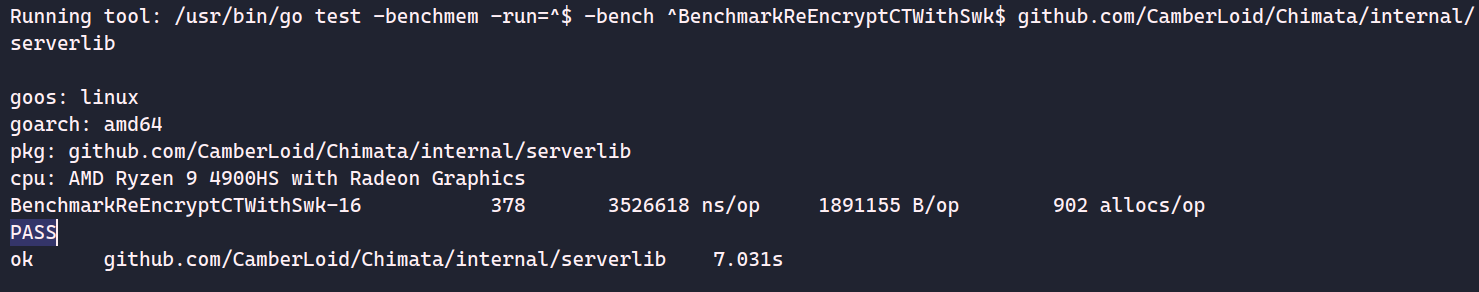
\includegraphics[width=0.8\linewidth]{./Figures/Bench_ReEncrypt.png}
    \caption{密文重加密的基准测试输出}\label{Fig:bench_reencrypt}
\end{figure}

在同态运算方面,本文所提出的方案涉及到的同态运算主要为密态余额的更新,即在交易完成后进行的对发送方和接收方的余额的更新,涉及到密文之间的同态加法和密文与明文常数的同态乘法。因此,笔者也对这部分被封装的同态运算函数进行了性能基准测试。测试方法为执行以下命令:

\begin{minted}{shell}
    $ /usr/bin/go test -benchmem -run=^$ \
    -bench ^BenchmarkGetUpdated\* \
    github.com/CamberLoid/Chimata/internal/serverlib
\end{minted}

收集到的测试数据如表\ref{Tab:CTUpdate}所示,测试数据显示,对于单笔交易,平均每次对转出方和转入方的余额进行更新的时间总和约为 4.5 ms。

\begin{table}[h]
    \centering
    \begin{tabular}{|l|c|c|}
        \hline
        测试函数 & 测试次数 & 平均单次时间开销 \\
        \hline
        BenchmarkGetUpdatedSenderBalance & 530 & 2.38 ms \\
        \hline
        BenchmarkGetUpdatedReceiptBalance & 550 & 2.33 ms \\
        \hline
        BenchmarkGetUpdatedBalance & 260 & 4.55 ms \\
        \hline
    \end{tabular}
    \caption{测试数据:同态密文更新的时间开销} \label{Tab:CTUpdate}
\end{table}

笔者亦对服务端相关数据库操作的时间开销进行。测试方法为服务端方面对每个数据库操作函数的时间开销进行测量,并记录总共操作的交易,在程序接收 SIGINT 信号退出时于日志中输出总时间开销除以总处理交易。计算过程如\eqref{eq:database_measure}所示。在执行前文交易基准测试后,使用 \texttt{Ctrl-C} 终止服务端,服务端输出如图\ref{Fig:bench_database_perf}所示。

\begin{equation} \label{eq:database_measure}
    \textrm{平均数据库操作时间} = \frac{\textrm{数据库操作总时间}}{\textrm{处理的交易笔数}}
\end{equation}

\begin{minted}{go}
    var _start time.Timer
    // 无关内容
    _start = time.Now()
    // 数据库操作
    DurationDatabaseOpr += time.Since(_start)
\end{minted}

\begin{figure}[h]
    \centering
    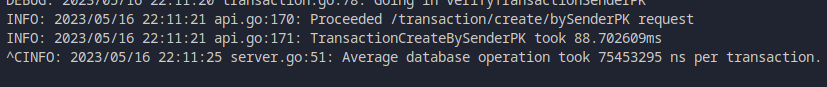
\includegraphics[width=0.8\linewidth]{./Figures/Test_Database_Perf.png}
    \caption{服务端关于数据库操作的输出} \label{Fig:bench_database_perf}
\end{figure}

由输出可知,对于每次交易,数据库操作开销,包括查询和写入,平均时间开销为 75.5 ms。

\subsubsection{测试结果分析}

\begin{table}[h]
    \begin{tabular}{|l|c|c|c|c|}
        \hline
        类别 & 单笔交易 & 加解密与重加密 & 密态余额更新 & 数据库操作 \\
        \hline
        平均消耗时间 & 105 ms & 15 ms & 4.5 ms & 75.5 ms \\ 
        \hline
        百分比 & 100.0\% & 14.2\% & 4.3\% & 71.9\% \\
        \hline
    \end{tabular}
    \caption{各部分时间开销与单笔交易开销的关系} \label{Tab:time_comsumption}
\end{table}

综合上述测试结果,服务端对单笔交易两个不同的方法的平均处理和返回时间约为 105 ms,其中 CKKS 方案的密码学相关函数占比约为 20\%,可以认为在选择的安全参数下,本文的同态加密核心部分工作性能良好。而 CKKS 方案的密码学函数以外的时间开销以数据库操作为主,占据了单笔交易的大部分处理时间,约为 70\%,未来的优化方向可以从这方面入手。其他开销约占比 10\%,包括了网络交互开销和签名验证开销等。

此外也可以从测试结果观察到,测试总时间开销相对服务端平均每笔交易的处理时间开销的总和要高,在连续处理交易笔数较少的时候尤为明显。笔者推测该额外开销是由 Golang 工具链自带的测试模组本身开销导致,具体而言包括了测试模块初始化开销,以及测试模块对单个测试的管理的开销等。这些开销是不可避免的,并被 Golang 工具计算在了总时间开销内。

\subsection{交易的空间开销测试}

本小节对服务端在处理交易信息后,其存储的密文的数据库大小,即服务端的空间开销进行评估。测试方法为,通过基准测试函数 \verb|CreateTransferJobByReceiptPK| 和对应的使用发送方公钥加密版本,令服务端连续处理至多 1000 笔不同的交易后,对其数据库大小进进行测算。每次进行新的测试循环前,都会对数据库文件进行删除并重新启动客户端,让服务端生成新的数据库文件。对实验结果进行收集后,使用 Python 模组 matplotlib 绘制折线图。结果如图\ref{Fig:graph_database_size}所示。

\begin{figure}[h]
    \centering
    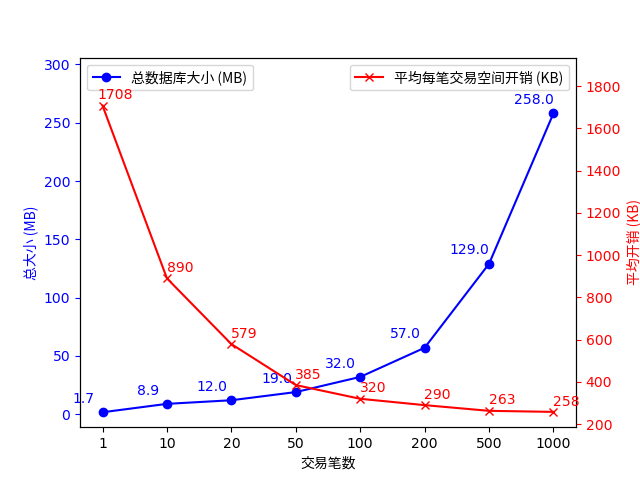
\includegraphics[width=0.8\linewidth]{./Figures/matplots/Bench_DatabaseSize.png}
    \caption{交易方案的空间开销测试数据} \label{Fig:graph_database_size}
\end{figure}

由实验结果可知,当连续处理交易笔数越多时,总数据库大小增加,平均每笔交易的空间开销不断降低,趋近于当交易笔数为 1000 时的约 258 KB 每笔交易。可以推算,每 1 GB 空间可以存储约 4000 笔交易信息。由于本文实现并未引入数据压缩,可以预测若引入数据压缩算法的话,能够取得更加优秀的结果。可惜的是,目前对基于全同态加密的交易方案的空间开销评估的现有研究较少,因此无法和其他方案进行对比。但考虑到目前计算机存储成本越来越低,可以认为本文所提出的服务端实现具有较高的空间效率,具有可实现性。

此外,可以注意到当交易笔数较少时,数据库所占用空间虽小,但平均每笔交易的空间开销较大,笔者推测这可能是数据库同时存储了元数据、配置数据和用户数据的原因。

\section{本章小结}

为测试提出方案的性能,本章对基于同态加密的用户交易金额隐私保护交易方案中的密码学部分以及交易处理部分,借助 Golang 工具链进行了基准测试。实验结果表明,在预设的安全参数下,本文所提出的交易方案,在密码学部分具有较高的效率;从总体来看,本方案的单次交易性能也符合预期,在实际应用中具有高效性。
